\section{Динамическое программирование}\label{valueiterationsection}

\subsection{Метод простой итерации}

%\needspace{6\baselineskip}
\begin{wrapfigure}{r}{0.45\textwidth}
\vspace{-1cm}
\centering
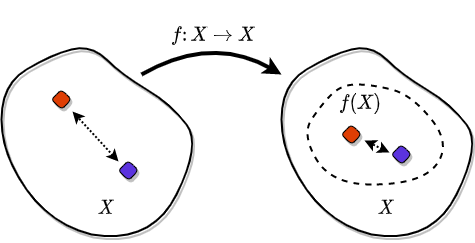
\includegraphics[width=0.4\textwidth]{Images/ContractionMapping.png}
\vspace{-1cm}
\end{wrapfigure}

Хотим научиться решать уравнения Беллмана, но мы видим, что уравнения оптимальности Беллмана нелинейные. Тем не менее, они имеют весьма определённый вид и, как мы сейчас увидим, обладают очень приятными свойствами. Нам понадобится несколько понятий внезапно из функана о том, как решать системы нелинейных уравнений вида $x \HM= f(x)$.

\begin{definition}
Оператор $f \colon X \to X$ называется \emph{сжимающим} (contraction) с коэффициентом сжатия $\gamma < 1$ по некоторой метрике $\rho$, если $\forall x_1, x_2 \colon$
$$\rho(f(x_1), f(x_2)) < \gamma \rho(x_1, x_2)$$
\end{definition}

\begin{definition}
Точка $x \in X$ для оператора $f \colon X \to X$ называется \emph{неподвижной} (fixed point), если
$$x = f(x)$$
\end{definition}

\begin{definition}
Построение последовательности $x_{k+1} = f(x_k)$ для начального приближения $x_0 \in X$ называется методом \emph{простой итерации} (point iteration) решения уравнения $x = f(x)$.
\end{definition}

\begin{theorem}[Теорема Банаха о неподвижной точке]\label{Banach}
В полном\footnote{любая фундаментальная последовательность имеет предел} метрическом пространстве $X$ у сжимающего оператора $f \colon X \to X$ существует и притом ровно одна неподвижная точка $x^*$, причём метод простой итерации сходится к ней из любого начального приближения.
\begin{proof}[Сходимость метода простой итерации] Пусть $x_0$ --- произвольное, $x_{k+1} = f(x_k)$. Тогда для любого $k > 0$:
\begin{equation}
\begin{aligned}\label{onestepcontraction}
\rho(x_k, x_{k+1}) = \{ \text{определение $x_k$} \} &= \rho(f(x_{k-1}), f(x_k)) \le \\ 
\le \{ \text{свойство сжатия} \} &\le \gamma \rho(x_{k-1}, x_k) \le \dots \le \\
\le \{ \text{аналогичным образом} \} &\le \dots \le \gamma^k \rho(x_0, x_1)
\end{aligned}
\end{equation}

Теперь посмотрим, что произойдёт после применения оператора $f$ $n$ раз:
\begin{align*}
\rho(x_k, x_{k + n}) &\le \\
\{ \text{неравенство треугольника} \}
&\le \rho(x_k, x_{k + 1}) + \rho(x_{k+1}, x_{k+2}) + \dots + \rho(x_{k + n - 1}, x_{k + n}) \le \\
\le \{ \text{\eqref{onestepcontraction}} \} 
&\le (\gamma^k + \gamma^{k+1} + \dots \gamma^{k+n-1}) \rho(x_0, x_1) \le \\
\le \{ \text{геом. прогрессия} \} &\le \frac{\gamma^k}{1 - \gamma} \rho(x_0, x_1) \xrightarrow{k \to \infty} 0
\end{align*}

Итак, последовательность $x_k$ --- фундаментальная, и мы специально попросили такое метрическое пространство (<<полное>>), в котором обязательно найдётся предел $x^* \coloneqq \lim\limits_{k \to \infty} x_k$.
\end{proof}
\begin{proof}[Существование неподвижной точки] Покажем, что $x^*$ и есть неподвижная точка $f$, то есть покажем, что наш метод простой итерации конструктивно её построил. Заметим, что для любого $k > 0$:
\begin{align*}
\rho(x^*, f(x^*)) &\le \\
\le \{ \text{неравенство треугольника} \} &\le \rho(x^*, x_k) + \rho(x_k, f(x^*)) = \\
= \{ \text{определение $x_k$} \} &= \rho(x^*, x_k) + \rho(f(x_{k-1}), f(x^*)) \le \\ 
\le \{ \text{свойство сжатия} \} &\le \rho(x^*, x_k) + \gamma \rho(x_{k-1}, x^*)
\end{align*}
Устремим $k \to \infty$; слева стоит константа, не зависящая от $k$. Тогда расстояние между $x_k$ и $x^*$ устремится к нулю, ровно как и между $x_{k-1}, x^*$ поскольку $x^*$ --- предел $x_k$. Значит, константа равна нулю, $\rho(x^*, f(x^*)) = 0$, следовательно, $x^* = f(x^*)$.
\end{proof}

\begin{proof}[Единственность] Пусть $x_1, x_2$ --- две неподвижные точки оператора $f$. Ну тогда:
$$\rho(x_1, x_2) = \rho(f(x_1), f(x_2)) \le \gamma \rho(x_1, x_2)$$
Получаем, что такое возможно только при $\rho(x_1, x_2) = 0$, то есть только если $x_1$ и $x_2$ совпадают.
\end{proof}
\end{theorem}

% TODO: пример, иллюстрация

\subsection{Policy Evaluation}

Вернёмся к RL. Известно, что $V^\pi$ для данного MDP и фиксированной политики $\pi$ удовлетворяет уравнению Беллмана \eqref{VV}. Для нас это система уравнений относительно значений $V^\pi(s)$. $V^\pi(s)$ --- объект (точка) в функциональном пространстве $\St \to \R$.

Будем решать её методом простой итерации\footnote{вообще говоря, это система линейных уравнений относительно значений $V^\pi(s)$, которую в случае табличных MDP можно решать любым методом решения СЛАУ. Однако, дальнейшие рассуждения через метод простой итерации обобщаются, например, на случай непрерывных пространств состояний $\St \subseteq \R^n$.}. Для этого определим оператор $\B$, то есть преобразование из одной функции $\St \to \R$ в другую. На вход этот оператор принимает функцию $V$ и выдаёт некоторую другую функцию от состояний $\B V$. Чтобы задать выход оператора, нужно задать значение выходной функции в каждом $s \in \St$; это значение мы будем обозначать $\left[\B V\right] (s)$ (квадратные скобки позволяют не путать применение оператора с вызовом самой функции) и определим его как правую часть решаемого уравнения \eqref{VV}. Итак:

\begin{definition}
Введём \emph{оператор Беллмана} (Bellman operator) как
$$\left[\B V\right] (s) \coloneqq \E_{a} \left[ r(s, a) + \gamma \E_{s'} V^\pi(s') \right]$$
\end{definition}

Также нам нужна метрика на множестве функций $\St \to \R$; возьмём
$$d_\infty(V_1, V_2) \coloneqq \max_s | V_1(s) - V_2(s) |$$

\begin{theorem}
Если $\gamma < 1$, оператор $\B$ --- сжимающий с коэффициентом сжатия $\gamma$.
\beginproof
\begin{align*}
&d_\infty(\B V_1, \B V_2) = \max_s \left| [\B V_1](s) - [\B V_2](s) \right| = \\
&= \{ \text{подставляем значение операторов, т.е. правые части решаемого уравнения} \} = \\
&= \max_s \left| \E_{a} \left[ r(s, a) + \gamma \E_{s'} V_1^\pi(s') \right] - \E_{a} \left[ r(s, a) + \gamma \E_{s'} V_2^\pi(s') \right] \right| = \\
&= \{ \text{слагаемые $r(s, a)$ сокращаются} \} = \\
&= \gamma \max_s \left| \E_{a} \E_{s'} \left[ V_1^\pi(s') - V_2^\pi(s') \right] \right| \le \\
&\le \{ \text{используем свойство $\E_x f(x) \le \max\limits_x f(x)$ \footnotemark[1] } \} \le \\
&\le \gamma \max_s \max_{s'} \left| V_1^\pi(s') - V_2^\pi(s') \right| = \gamma d_\infty( V_1, V_2 ) \tagqed
\end{align*}
\end{theorem}
\footnotetext[1]{нет, через согласованные нормы стохастических несимметричных матриц, наверное, тоже можно...}

Итак, мы попали в теорему Банаха, и значит, мы гарантированно сойдёмся к единственной неподвижной точке. По построению мы знаем, что $V^\pi(s)$ такова, что $\B V^\pi = V^\pi$ (это и есть уравнение Беллмана), поэтому к ней и придём.

Обсудим, что случится в ситуации, когда $\gamma = 1$; напомню, что в таких ситуациях мы требовали эпизодичность сред, с гарантиями завершения всех эпизодов за $T^{\max}$ шагов. Оператор Беллмана формально сжатием являться уже не будет, и мы не подпадаем под теорему, поэтому этот случай придётся разобрать отдельно.

\begin{theoremBox}[label=th:policyevalepisodic]{}
В эпизодичных средах метод простой итерации сойдётся к единственному решению уравнений Беллмана не более чем за $T^{\max}$ шагов даже при $\gamma = 1$.
\begin{proof}
Мы уже доказывали теорему \ref{th:episodicmdpistree}, что граф таких сред является деревом. Будем говорить, что состояние $s$ находится на ярусе $T$, если при старте из $s$ у любой стратегии есть гарантии завершения за $T$ шагов. Понятно, что для состояния $s$ на ярусе $T$ верно, что $\forall s', a$, для которых $p(s' \mid s, a) > 0$, ярус $s'$ не превосходит $T - 1$. 

Осталось увидеть, что на $k$-ой итерации метода простой итерации вычисляет точные значения $V^{\pi}(s)$ для всех состояний на ярусах до $k$: действительно, покажем по индукции. Считаем, что терминальные состояния имеют нулевой ярус; а на $k$-ом шаге при обновлении $V^{\pi}(s)$ для $s$ на $k$-ом ярусе в правой части уравнения Беллмана будет стоять мат.~ожидание по $s'$ с ярусов до $k - 1$-го, для которых значение по предположению индукции уже посчитано точно.

Соответственно, за $T^{\max}$ шагов точные значения распространятся на все состояни, и конструктивно значения определены однозначно.
\end{proof}
\end{theoremBox}

\begin{remark}
Если $\gamma = 1$, а среда неэпизодична (такие MDP мы не допускали к рассмотрению), метод простой итерации может не сойтись, а уравнения Беллмана могут в том числе иметь бесконечно много решений. Пример подобного безобразия. Пусть в MDP без терминальных состояний с нулевой функцией награды (где, очевидно, $V^{\pi}(s) \HM= 0$ для всех $\pi, s$) мы проинициализировали $V^{\pi}(s) \HM= 100$ во всех состояниях $s$. Тогда при обновлении наша аппроксимация не будет меняться: мы уже в неподвижной точке уравнений Беллмана. В частности поэтому на практике практически никогда не имеет смысл выставлять $\gamma \HM = 1$, особенно в сложных средах, где, может быть, даже и есть эпизодичность, но, тем не менее, есть <<похожие состояния>>: они начнут работать <<как петли>>, когда мы перейдём к приближённым методам динамического программирования в дальнейшем.
\end{remark}

\begin{proposition}
Если некоторая функция $\tilde{V} \colon \St \to \R$ удовлетворяет уравнению Беллмана \eqref{VV}, то $\tilde{V} \equiv V^\pi$.
\end{proposition}

Мы научились решать задачу \emph{оценивания стратегии} (Policy Evaluation): вычислять значения оценочной функции по данной стратегии $\pi$ в ситуации, когда мы знаем динамику среды. На практике мы можем воспользоваться этим результатом только в \emph{<<табличном>> случае} (tabular RL), когда пространство состояний и пространство действий конечны и достаточно малы, чтобы все пары состояние-действие было возможно хранить в памяти компьютера и перебирать за разумное время. В такой ситуации $V^\pi(s)$ --- конечный векторочек, и мы умеем считать оператор Беллмана и делать обновления $V_{k+1} = \B V_k$.

\begin{algorithm}[label=policyevaluation]{Policy Evaluation}
\textbf{Вход:} $\pi(a \mid s)$ --- стратегия \\
\textbf{Гиперпараметры:} $\eps$ --- критерий останова.

\vspace{0.3cm}
Инициализируем $V_0(s)$ произвольно для всех $s \in \St$. \\
\textbf{На $k$-ом шаге:}
\begin{enumerate}
    \item $\forall s \colon V_{k+1}(s) \coloneqq \E_{a} \left[ r(s, a) + \gamma \E_{s'} V_k(s')\right]$
    \item \textbf{критерий останова:} $\max\limits_s |V_k(s) - V_{k+1}(s)| < \eps$
\end{enumerate}

\vspace{0.3cm}
\textbf{Выход:} $V_k(s)$
\end{algorithm}

\begin{exampleBox}[label=ex:pe, righthand ratio=0.3, sidebyside, sidebyside align=center, lower separated=false]{}
Проведём оценивание стратегии, случайно выбирающей, в какую сторону ей пойти, с $\gamma = 0.9$. Угловые клетки с ненулевой наградой терминальны; агент остаётся в той же клетке, если упирается в стенку. На каждой итерации отображается значение текущего приближения $V^{\pi}(s)$.

\tcblower
%\vspace{-0.3cm}
\animategraphics[controls, width=0.9\linewidth]{1}{Images/PE/policyeval}{0}{9}
\end{exampleBox}

Итак, мы научились считать $V^\pi$ в предположении известной динамики среды. Полностью аналогичное рассуждение верно и для уравнений QQ \eqref{QQ}; то есть, расширив набор переменных, в табличных MDP можно методом простой итерации находить $Q^{\pi}$ и <<напрямую>>. Пока модель динамики среды считается известной, это не принципиально: мы можем посчитать и Q-функцию через V-функцию по формуле QV \eqref{QV}.


% Удобен схожий алгоритм\footnote{не могу найти внятного объяснения, почему этот переход ничего не ломает, но кажется, что это так.}, позволяющий не хранить целиком $V_k$ для расчёта $V_{k+1}$, а проводить все вычисления по одной таблице:

% \begin{algorithm}{Iterative Policy Evaluation}
% \textbf{Гиперпараметры: } $\varepsilon$ --- критерий останова. \\
% \textbf{Вход:} $\pi(a \mid s)$ --- стратегия.

% \vspace{0.3cm}
% Инициализируем $V(s)$ произвольно для всех $s \in \St$. \\
% \textbf{На $k$-ом шаге:}
% \begin{enumerate}
%     \item храним максимальное изменение на данном шаге $\delta_k \coloneqq 0$
%     \item \textbf{перебираем $s \in \St$:}
%     \begin{itemize}
%         \item сохраняем старое значение $\nu \coloneqq V(s)$
%         \item обновляем $V(s) \leftarrow \E_{a} \left[ r(s, a) + \gamma \E_{s'} V(s')\right]$
%         \item обновляем максимальное изменение $\delta_k \leftarrow \max \left( \delta_k, |V(s) - \nu| \right)$
%     \end{itemize}
%     \item \textbf{критерий останова:} $\delta_k < \varepsilon$
% \end{enumerate}

% \vspace{0.3cm}
% \textbf{Выход:} $V(s)$
% \end{algorithm}

\subsection{Value Iteration}

Теорема Банаха позволяет аналогично Policy Evaluation (алг. \ref{policyevaluation}) решать уравнения оптимальности Беллмана \eqref{Q*Q*} через метод простой итерации. Действительно, проведём аналогичные рассуждения (мы сделаем это для $Q^*$, но совершенно аналогично можно было бы сделать это и для $V^*$):

\begin{definition}
Определим \emph{оператор оптимальности Беллмана} (Bellman optimality operator, Bellman control operator) $\B^*$:
$$\left[\B^* Q\right] (s, a) \coloneqq r(s, a) + \gamma \E_{s'} \max_{a'}Q(s', a')$$
\end{definition}

В качестве метрики на множестве функций $\St \times \A \to \R$ аналогично возьмём
$$d_\infty(Q_1, Q_2) \coloneqq \max_{s, a} | Q_1(s, a) - Q_2(s, a) |$$

Нам понадобится следующий факт:
\begin{proposition}\,
\begin{equation}\label{diffmax}
| \max_x f(x) - \max_x g(x) | \le \max_x | f(x) - g(x) |
\end{equation}
\begin{proof}
Рассмотрим случай $\max\limits_x f(x) \HM> \max\limits_x g(x)$. Пусть $x^*$ --- точка максимума $f(x)$. Тогда:
\begin{align*}
    \max_x f(x) - \max_x g(x) \le f(x^*) - \max_x g(x) \le f(x^*) - g(x^*) \le \max_x | f(x) - g(x) |
\end{align*}
Второй случай рассматривается симметрично.
\end{proof}
\end{proposition}

\begin{theorem}
Если $\gamma < 1$, оператор $\B^*$ --- сжимающий.
\beginproof
\begin{align*}
&d_\infty(\B^*Q_1, \B^*Q_2) = \max_{s, a} \left| [\B^*Q_1](s, a) - [\B^*Q_2](s, a) \right| = \\
&= \{ \text{подставляем значения операторов, т.е. правые части решаемой системы уравнений} \} = \\
&= \max_{s, a} \left| \left[ r(s, a) + \gamma \E_{s'} \max_{a'} Q_1(s', a') \right] - \left[ r(s, a) + \gamma \E_{s'} \max_{a'} Q_2(s', a') \right] \right| = \\
&= \{ \text{слагаемые $r(s, a)$ сокращаются} \} = \\
&= \gamma \max_{s, a} \left| \E_{s'} \left[ \max_{a'} Q_1(s', a') - \max_{a'} Q_2(s', a') \right] \right| \le \\
&\le \{ \text{используем свойство $\E_x f(x) \le \max\limits_x f(x)$} \} \le \\
&\le \gamma \max_{s, a} \max_{s'} \left| \max_{a'} Q_1(s', a') - \max_{a'} Q_2(s', a') \right| = \\
&\le \{ \text{используем свойство максимумов \eqref{diffmax}} \} \le \\
& \le \gamma \max_{s, a} \max_{s'} \max_{a'} \left| Q_1(s', a') - Q_2(s', a') \right| \le \\
&= \{\text{внутри стоит определение $d_\infty(Q_1, Q_2)$, а от внешнего максимума ничего не зависит}\} = \\
&= \gamma d_\infty( Q_1, Q_2 )   \tagqed
\end{align*}
\end{theorem}

\begin{theorem}
В эпизодичных средах метод простой итерации сойдётся к единственному решению уравнений оптимальности Беллмана не более чем за $T^{\max}$ шагов даже при $\gamma = 1$.
\begin{proof} Полностью аналогично доказательству теоремы \ref{th:policyevalepisodic}.
\end{proof}
\end{theorem}

\begin{proposition}
Если некоторая функция $\tilde{Q} \colon \St \times \A \to \R$ удовлетворяет уравнению оптимальности Беллмана \eqref{Q*Q*}, то $\tilde{Q} \equiv Q^*$.
\end{proposition}

\begin{proposition}
Метод простой итерации сходится к $Q^*$ из любого начального приближения.
\end{proposition}

Вообще, если известна динамика среды, то нам достаточно решить уравнения оптимальности для $V^*$ --- это потребует меньше переменных. Итак, в табличном случае мы можем напрямую методом простой итерации решать уравнения оптимальности Беллмана и в пределе сойдёмся к оптимальной оценочной функции, которая тут же даёт нам оптимальную стратегию.

\begin{algorithm}[label=valueiteration]{Value Iteration}
\textbf{Вход:} $\varepsilon$ --- критерий останова.

\vspace{0.3cm}
Инициализируем $V^*_0(s)$ произвольно для всех $s \in \St$. \\
\textbf{На $k$-ом шаге:}
\begin{enumerate}
    \item для всех $s$: $V^*_{k+1}(s) \leftarrow \max\limits_a \left[ r(s, a) + \gamma \E_{s'} V^*_k(s')\right]$
    \item \textbf{критерий останова:} $\max\limits_{s} | V^*_{k+1}(s) - V^*_k(s) | < \varepsilon$
\end{enumerate}

\vspace{0.3cm}
\textbf{Выход:} $\pi(s) \coloneqq \argmax\limits_a \left[ r(s, a) + \gamma \E_{s'} V^*(s')\right]$
\end{algorithm}

\needspace{7\baselineskip}
\begin{wrapfigure}{r}{0.35\textwidth}
%\vspace{-0.3cm}
\centering
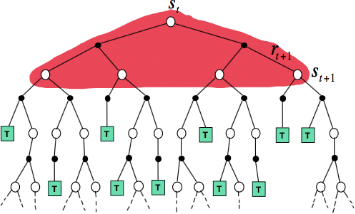
\includegraphics[width=0.3\textwidth]{Images/DP_backup.png}
%\vspace{-0.3cm}
\end{wrapfigure}

Итак, мы придумали наш первый табличный алгоритм планирования --- алгоритм, решающий задачу RL в условиях известной модели среды. На каждом шаге мы обновляем (<<бэкапим>>) нашу текущую аппроксимацию V-функции на её \emph{одношаговое приближение} (one-step approximation): смотрим на один шаг в будущее ($r, a, s'$) и приближаем всё остальное будущее текущей же аппроксимацией. Такой <<бэкап динамического программирования>> (dynamic programming backup, DP-backup) --- обновление <<бесконечной ширины>>: мы должны перебрать все возможные варианты следующего одного шага, рассмотреть все свои действия (по ним мы возьмём максимум) и перебрать всевозможные ответы среды --- $s'$ (по ним мы должны рассчитать мат.ожидание). Поэтому этот алгоритм в чистом виде напоминает то, что обычно и понимается под словами <<динамическое программирование>>: мы <<раскрываем дерево игры>> полностью на один шаг вперёд.

\begin{exampleBox}[righthand ratio=0.3, sidebyside, sidebyside align=center, lower separated=false]{}
Решим задачу из примера \ref{ex:pe}, $\gamma = 0.9$; на каждой итерации отображается значение текущего приближения $V^{*}(s)$. В конце концов в силу детермнированности среды станет понятно, что можно избежать попадания в терминальное -1 и кратчайшим путём добираться до терминального +1.

\tcblower
%\vspace{-0.3cm}
\animategraphics[controls, width=0.9\linewidth]{1}{Images/VI/valueiter}{0}{9}
\end{exampleBox}

% \begin{algorithm}[label=valueiteration]{Value Iteration}
% \textbf{Вход:} $\varepsilon$ --- критерий останова.

% \vspace{0.3cm}
% Инициализируем $V^*(s)$ произвольно для всех $s \in \St$. \\
% \textbf{На $k$-ом шаге:}
% \begin{enumerate}
%     \item храним максимальное изменение $\delta_k \coloneqq 0$
%     \item \textbf{перебираем $s \in \St$:}
%     \begin{itemize}
%         \item сохраняем старое значение $\nu \coloneqq V^*(s)$
%         \item обновляем $V^*(s) \leftarrow \max\limits_a \left[ r(s, a) + \gamma \E_{s'} V^*(s')\right]$
%         \item обновляем максимальное изменение $\delta_k \leftarrow \max \left( \delta_k, |V^*(s) - \nu| \right)$
%     \end{itemize}
%     \item \textbf{критерий останова:} $\delta_k < \varepsilon$
% \end{enumerate}

% \vspace{0.3cm}
% \textbf{Выход:} $\pi(s) \coloneqq \argmax\limits_a \left[ r(s, a) + \gamma \E_{s'} V^*(s')\right]$
% \end{algorithm}



\subsection{Policy Iteration}

\needspace{7\baselineskip}
\begin{wrapfigure}{r}{0.35\textwidth}
\vspace{-1cm}
\centering
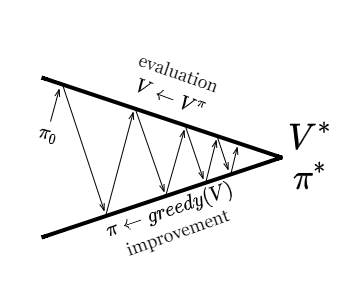
\includegraphics[width=0.3\textwidth]{Images/PI_basic.png}
\vspace{-1cm}
\end{wrapfigure}

Мы сейчас в некотором смысле <<обобщим>> Value Iteration и придумаем более общую схему алгоритма планирования для табличного случая.

Для очередной стратегии $\pi_k$ посчитаем её оценочную функцию $Q^{\pi_k}$, а затем воспользуемся теоремой Policy Improvement \ref{th:policyimprovement} и построим стратегию лучше; например, жадно:
$$\pi_{k+1}(s) \coloneqq \argmax\limits_{a} Q^{\pi_k}(s, a)$$

Тогда у нас есть второй алгоритм планирования, который, причём, перебирает детерминированные стратегии, обладающие свойством монотонного возрастания качества: каждая следующая стратегия не хуже предыдущей. Он работает сразу в классе детерминированных стратегий, и состоит из двух этапов:
\begin{itemize}
    \item \textbf{Policy Evaluation}: вычисление $Q^\pi$ для текущей стратегии $\pi$;
    \item \textbf{Policy Improvement}: улучшение стратегии $\pi(s) \leftarrow \argmax\limits_a Q^\pi(s, a)$;
\end{itemize}

При этом у нас есть гарантии, что когда алгоритм <<останавливается>> (не может провести Policy Improvement), то он находит оптимальную стратегию. Будем считать\footnote{считаем, что аргмакс берётся однозначно для любой Q-функции: в случае, если в $\Argmax$ содержится более одного элемента, множество действий как-то фиксированно упорядочено, и берётся действие с наибольшим приоритетом.}, что в такой момент остановки после проведения Policy Improvement наша стратегия не меняется: $\pi_{k+1} \equiv \pi_k$.

\begin{theorem}
В табличном сеттинге Policy Iteration завершает работу за конечное число итераций.
\begin{proof}
Алгоритм перебирает детерминированные стратегии, и, если остановка не происходит, каждая следующая лучше предыдущей:
$$\pi_k \succ \pi_{k-1} \succ \dots \succ \pi_0$$
Это означает, что все стратегии в этом ряду различны. Поскольку в табличном сеттинге число состояний и число действий конечны, детерминированных стратегий конечное число; значит, процесс должен закончится.
\end{proof}
\end{theorem}

\begin{algorithm}[label=policyiteration]{Policy Iteration}
\textbf{Гиперпараметры:} $\eps$ --- критерий останова для процедуры $\operatorname{PolicyEvaluation}$.

\vspace{0.3cm}
Инициализируем $\pi_0(s)$ произвольно для всех $s \in \St$. \\
\textbf{На $k$-ом шаге:}
\begin{enumerate}
    \item $V^{\pi_k} \coloneqq \operatorname{PolicyEvaluation}(\pi_k, \eps)$
    \item $Q^{\pi_k}(s, a) \coloneqq r(s, a) + \gamma \E_{s'} V^{\pi_k}(s')$
    \item $\pi_{k+1}(s) \coloneqq \argmax\limits_a Q^{\pi_k}(s, a)$
    \item \textbf{критерий останова:} $\pi_k \equiv \pi_{k+1}$
\end{enumerate}
\end{algorithm}

\begin{exampleBox}[righthand ratio=0.5, sidebyside, sidebyside align=center, lower separated=false]{}
Решим задачу из примера \ref{ex:pe}, $\gamma = 0.9$; на каждой итерации слева отображается $V^{\pi_k}(s)$; справа улучшенная $\pi_{k+1}$. За 4 шага алгоритм сходится к оптимальной стратегии.

\tcblower
%\vspace{-0.3cm}
\animategraphics[controls, width=\linewidth]{1}{Images/PI/policyiter}{0}{3}
\end{exampleBox}

\subsection{Generalized Policy Iteration}

Теперь поймём, почему Policy Iteration --- более общая схема. Будем считать, что процедуру оценивания стратегии, этап Policy Evaluation, мы решаем методом простой итерации. Вообще говоря, процедура предполагает бесконечное число шагов, и на практике нам нужно когда-то остановиться; теоретически мы считаем, что доводим вычисления до некоторого критерия останова, когда значения вектора не меняются более чем на некоторую погрешность $\eps > 0$. 

\needspace{7\baselineskip}
\begin{wrapfigure}{r}{0.35\textwidth}
\vspace{-1.2cm}
\centering
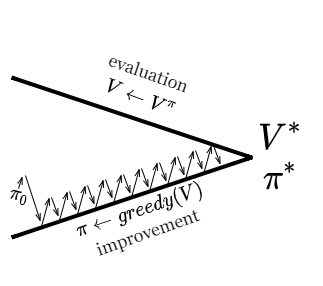
\includegraphics[width=0.3\textwidth]{Images/VI_basic.png}
\vspace{-1cm}
\end{wrapfigure}

Но рассмотрим такую, пока что, эвристику: давайте останавливать Policy Evaluation после ровно $N$ шагов, а после обновления стратегии не начинать оценивать $\pi_{k+1}$ с нуля, а использовать $V^{\pi_{k}}$ в качестве инициализации. Мы формально потеряем гарантии улучшения стратегии на этапе Policy Improvement, поэтому останавливать алгоритм после того, как стратегия не изменилась, уже нельзя: возможно, после следующих $N$ шагов обновления оценочной функции, аргмакс поменяется. Тогда наш алгоритм примет следующий вид: 

\begin{algorithm}[label=generalizedpolicyiteration]{Generalized Policy Iteration}
\textbf{Гиперпараметры:} $N$ --- количество шагов.

\vspace{0.3cm}
Инициализируем $\pi(s)$ произвольно для всех $s \in \St$. \\
\textbf{На $k$-ом шаге:}
\begin{enumerate}
    \item \textbf{Повторить $N$ раз:}
    \begin{itemize}
        \item $\forall s \colon V^{\pi}(s) \leftarrow \E_{a} \left[ r(s, a) + \gamma \E_{s'} V^{\pi}(s')\right]$
    \end{itemize}
    \item $Q^{\pi}(s, a) \leftarrow r(s, a) + \gamma \E_{s'} V^{\pi}(s')$
    \item $\pi(s) \leftarrow \argmax\limits_a Q^{\pi}(s, a)$
\end{enumerate}
\end{algorithm}

\begin{proposition}
Generalized Policy Iteration (алг. \ref{generalizedpolicyiteration}) совпадает с Value Iteration (алг. \ref{valueiteration}) при $N \HM= 1$ и с Policy Iteration (алг. \ref{policyiteration}) при $N = \infty$.
\begin{proof}
Второе очевидно; увидим первое. При $N = 1$ наше обновление V-функции имеет следующий вид:
$$V^{\pi}(s) \leftarrow \E_{a} \left[ r(s, a) + \gamma \E_{s'} V^{\pi}(s') \right]$$
Вспомним, по какому распределению берётся мат.~ожидание $\E_a$: по $\pi$, которая имеет вид 
$$\pi(s) = \argmax\limits_a Q^{\pi}(s, a) = \argmax\limits_a \left[ r(s, a) + \gamma \E_{s'} V^{\pi}(s') \right]$$
Внутри аргмакса как раз стоит содержимое нашего мат.ожидания в обновлении V, поэтому это обновление выродится в
$$V^{\pi}(s) \leftarrow \max\limits_{a} \left[ r(s, a) + \gamma \E_{s'} V^{\pi}(s') \right]$$
Это в точности обновление из алгоритма Value Iteration.
\end{proof}
\end{proposition}

Итак, Generalized Policy Iteration при $N = 1$ и при $N = \infty$ --- это ранее разобранные алгоритмы, физический смысл которых нам ясен. В частности, теперь понятно, что в Value Iteration очередное приближение $Q^*_k$ можно рассматривать как приближение $Q^{\pi}$ для $\pi(s) \HM \coloneqq \argmax\limits_{a} Q^*_k(s, a)$; то есть в алгоритме хоть и не потребовалось в явном виде хранить <<текущую>> стратегию, она всё равно неявно в нём присутствует. 

Давайте попробуем понять, что происходит в Generalized Policy Iteration при промежуточных $N$. Заметим, что повторение $N$ раз метода простой итерации для решения уравнения $\B V^\pi \HM= V^\pi$ эквивалентно одной итерации метода простой итерации для решения уравнения $\B^N V^\pi \HM= V^\pi$ (где запись $\B^N$ означает повторное применение оператора $\B$ $N$ раз), для которого, очевидно, искомая $V^{\pi}$ также будет неподвижной точкой. Что это за оператор $\B^N$? 

В уравнениях Беллмана мы <<раскручивали>> наше будущее на один шаг вперёд и дальше заменяли оставшийся <<хвост>> на определение V-функции. Понятно, что мы могли бы раскрутить не на один шаг, а на $N$ шагов вперёд.

\begin{theorem}[$N$-шаговое уравнение Беллмана]\,
\begin{equation}\label{NstepBellman}
 V^{\pi}(s_0) = \E_{\Traj_{:N} \sim \pi \mid s_0} \left[ \sum_{t=0}^{N-1} \gamma^{t}r_t +  \gamma^N \E_{s_N} V^{\pi}(s_N) \right]   
\end{equation}
\begin{proof}[Доказательство по индукции]
Для получения уравнения на $N$ шагов берём $N-1$-шаговое и подставляем в правую часть раскрутку на один шаг из уравнения \eqref{VV}. Это в точности соответствует применению оператора Беллмана $N$ раз.
\end{proof}
\begin{proof}[Доказательство без индукции]
Для любых траекторий $\Traj$ верно, что
$$R(\Traj) = \sum_{t=0}^{N-1} \gamma^{t}r_t + \gamma^N R_N$$
Возьмём мат.ожидание $\E_{\Traj \sim \pi \mid s_0}$ слева и справа:
$$\E_{\Traj \sim \pi \mid s_0}R(\Traj) = \E_{\Traj \sim \pi \mid s_0} \left[ \sum_{t=0}^{N-1} \gamma^{t}r_t + \gamma^N R_N \right]$$
Слева видно определение V-функции. Справа достаточно разделить мат.ожидание на мат.ожидание по первым $N$ шагам и хвост:
$$V^{\pi}(s_0) = \E_{\Traj_{:N} \sim \pi \mid s_0} \left[ \sum_{t=0}^{N-1} \gamma^{t}r_t + \gamma^N \E_{s_N} \E_{\Traj_{N:} \sim \pi \mid s_N} R_N \right]$$
Осталось выделить справа во втором слагаемом определение V-функции.
\end{proof}
\end{theorem}

\begin{proposition}
$\B^N$ --- оператор с коэффициентом сжатия $\gamma^N$.
\beginproof
\begin{align*}
\rho(\B^N V_1, \B^N V_2) \le \gamma \rho (\B^{N-1} V_1, \B^{N-1} V_2) \le \dots \le \gamma^N \rho (V_1, V_2)   \tagqed
\end{align*}
\end{proposition}

Означает ли это, что метод простой итерации решения $N$-шаговых уравнений сойдётся быстрее? Мы по сути просто <<за один шаг>> делаем $N$ итераций метода простой итерации для решения обычного одношагового уравнения; в этом смысле, мы ничего не выигрываем. В частности, если мы устремим $N$ к бесконечности, то мы получим просто определение V-функции; формально, в правой части будет стоять выражение, вообще не зависящее от $V^{\pi}$, а коэффициент сжатия будет ноль, и метод простой итерации как бы сходится тут же за один шаг. Но для проведения этого шага нужно выинтегрировать все траектории --- <<раскрыть дерево полностью>>.

Но теперь у нас есть другой взгляд на Generalized Policy Iteration: мы чередуем одну итерацию решения $N$-шагового уравнения Беллмана с Policy Improvement-ом. Интуитивно, алгоритм стабилизируется, если оценочная функция будет удовлетворять уравнению Беллмана для текущей $\pi$ (иначе оператор $\B^N$ изменит значение функции), и если $\pi$ выбирает $\argmax\limits_{a} Q^{\pi}(s, a)$ из неё; то есть, при сходимости $\pi$ удовлетворит критерию оптимальности; существуют доказанные гарантии сходимости.

\needspace{7\baselineskip}
\begin{wrapfigure}{r}{0.35\textwidth}
\vspace{-0.7cm}
\centering
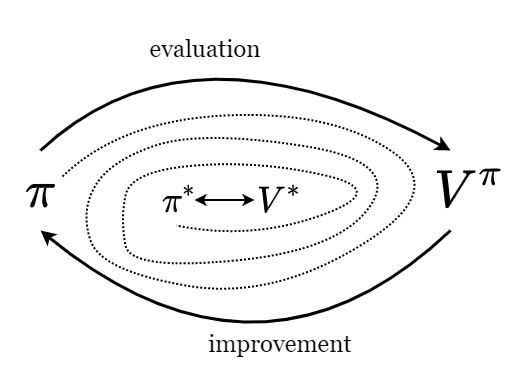
\includegraphics[width=0.3\textwidth]{Images/GPI.png}
\vspace{-0.5cm}
\end{wrapfigure}

Все алгоритмы, которые мы будем обсуждать далее, так или иначе подпадают под обобщённую парадигму <<оценивание-улучшение>>. Оценивание внутри алгоритма будет явно или неявно происходить при подсчёте каких-то оценок $V^{\pi}$ или $Q^{\pi}$ для текущей стратегии; Policy Improvement, как мы увидим, тоже будет выступать в разных формах. Например, самый простой способ решать задачу RL --- погенерировать несколько случайных стратегий и выбрать среди них лучшую --- тоже подпадает под эту парадигму: мы считаем Монте-Карло оценки значения $J(\pi)$ для нескольких разных стратегий (evaluation) и выбираем наилучшую стратегию (improvement). Мы далее начнём строить model-free алгоритмы, взяв наши алгоритмы планирования --- Policy Iteration и Value Iteration, --- и попробовав превратить их в табличные алгоритмы решения задачи.

% Исключительно для удобства нотации, покажем сходимость такого алгоритма в случае, если мы учим сразу Q-функцию, то есть проводим обновления следующего вида:
% $$Q^{\pi}(s_0, a_0) \leftarrow \E_{\Traj_{:N} \sim \pi \mid s_0, a_0} \left[ \sum_{t=0}^{N-1} \gamma^{t}r(s_t, a_t) + \gamma^N \E_{s_N} \E_{a_N} Q^{\pi}(s_N, a_N) \right],$$
% где $\pi(s) \coloneqq \argmax\limits_{a} Q^{\pi}(s, a)$, и, следовательно, обновление принимает вид:
% $$Q^{\pi}(s_0, a_0) \leftarrow \E_{\Traj_{:N} \sim \pi \mid s_0, a_0} \left[ \sum_{t=0}^{N-1} \gamma^{t}r(s_t, a_t) + \gamma^N \E_{s_N} \max\limits_{a_N} Q^{\pi}(s_N, a_N) \right],$$

% Можно ли к правой части применить нашу технику со сжимающими операторами? Выражение в правой части зависит как от нашей текущей аппроксимации $Q^{\pi}$, так и от стратегии $\pi$. 

% \begin{theorem}
% Generalized Policy Iteration, заключающийся в чередовании обновлений
% \begin{gather*}
% Q^{\pi} \leftarrow \B^{\pi}_N Q^{\pi} \\
% \pi(s) \leftarrow \argmax_{a} Q^{\pi}(s, a),
% \end{gather*}
% где
% $$\left[ \B^{\pi}_N Q^{\pi} \right](s, a) \coloneqq \E_{\Traj_{:N} \sim \pi \mid s_0, a_0} \left[ \sum_{t=0}^{N-1} \gamma^{t}r(s_t, a_t) + \gamma^N \E_{s_N} \max\limits_{a_N} Q^{\pi}(s_N, a_N) \right],$$
% сходится к $Q^*$.
% \begin{proof}
% Тонкость заключается в том, что наш оператор изменяется на каждом шаге (всё время меняется $\pi$). Однако, каждый оператор $\B^{\pi}_N$ является сжимающим в $\gamma^N$ раз: действительно,
% $$\B^{\pi}_N \equiv \B^{N-1} \B^*,$$
% а композиция сжимающих операторов есть также сжатие.

% Что за неподвижная точка у оператора $\B^{\pi}_N$ для фиксированной $\pi$? $Q^\pi$!
% \end{proof}
% \end{theorem}